\documentclass[openright,twoside,a4paper]{scrartcl}
\usepackage[ngerman]{babel}
\usepackage[utf8]{inputenc}
\usepackage[T1]{fontenc}
\usepackage{blindtext}
\usepackage{multicol}
\usepackage{url}
\usepackage{abstract}
\usepackage{graphicx}
\usepackage{caption}
\usepackage{wrapfig}
\usepackage{svg}

\clubpenalty10000
\widowpenalty10000
\displaywidowpenalty=10000

\author{Janek Boll}
\date{\today}

\newcommand{\blankpage}{
\newpage
\thispagestyle{empty}
\mbox{}
\newpage
}

%Eigene Bildumgebug definieren, weil das sonst seltsam ausgeht mit multicols
\newenvironment{Figure}
  {\par\medskip\noindent\minipage{\linewidth}}
  {\endminipage\par\medskip}

\begin{document}

    %römische Ziffern für die ersten Seiten
    \pagenumbering{roman}

    \titlehead{%
 {\setlength{\unitlength}{1mm}
  \begin{picture}(0,0)
    \put(-19,4){
\includegraphics{./aux/tuclogo}}
    \put(132,-269){
\includegraphics{./aux/rechteck}}
  \end{picture}}
}

\begin{titlepage}
    \makeatletter
    \@titlehead

    \begin{center}
        \vskip25mm
        
        \hspace*{-40mm}{\makebox[140mm]{\Large Projekt im Bachelor}}\par

        \vskip20mm

        \hspace*{-40mm}{\makebox[140mm]{\titlefont\huge Entwicklung von Sharing Boxen}}

        \vskip5mm

        \vskip1mm
        \hspace*{-40mm}{\makebox[140mm]{\titlefont\LARGE Protoyp zur elektronischen Öffnung von Boxen}}\par


        \vskip20mm

        \hspace*{-40mm}{\makebox[140mm]{\LARGE Janek Boll}}\par
        \hspace*{-40mm}{\makebox[140mm]{\large 447344}}\par

        \vskip10mm

        \hspace*{-40mm}{\makebox[140mm]{\Large \today}}\par

        \vskip33mm

        \hspace*{-40mm}{\makebox[140mm]{Institut für Informatik}}\par

        \hspace*{-40mm}{\makebox[140mm]{Prof. Dr. Andreas Rausch}}\par

        \vskip08mm
        
        \hspace*{-40mm}{\makebox[140mm]{betreut durch:}}\par

        \hspace*{-40mm}{\makebox[140mm]{Dirk Herrling, M. Sc.}}\par


    \end{center}
\end{titlepage}

    \newpage

    \setcounter{page}{1}

    \makeatletter

\cleardoublepage

\thispagestyle{empty}
\hskip 0mm
\vfill

\begin{center}
    \sffamily\bfseries\large Eidestattliche Erklärung
\end{center}

\bigskip\noindent Hiermit erkläre ich an Eides statt, dass ich die vorliegende Arbeit selbstständig verfasst und keine anderen als die angegebenen Hilfsmittel verwendet habe.\par
Mit einer Veröffentlichung der Arbeit in der Instituts- beziehungsweise Universitätsbibliothek bin ich einverstanden.\par

\bigskip\noindent Clausthal-Zellerfeld,~ \today\par
\vskip 10mm
\hfill \hrulefill\par
\hfill Janek Boll
\makeatother

    \newpage

    %Abstrakt zentrieren
    \topskip0pt
    \vspace*{\fill}
    \begin{abstract}
        asjdhajkshdakjshdaksjhdkajshdakjshdkajshdkasjhdkasjhdajkshdajshd
    \end{abstract}
    \vspace*{\fill}

    \newpage

    \tableofcontents

    \newpage

    %Arabische Ziffern für Hauptteil
    \pagenumbering{arabic}

    \section{Einführung}
        \subsection{Motivation}
            Mittelfristig sollen an der TU Clausthal elektronische Schließfächer eingeführt werden, die es Studierenden und Mitarbeitern der Universität ermöglichen, Gegenstände zu lagern und untereinander auszutauschen. Hierzu sollen die Teilnehmer in der Lage sein, Boxen, die an verschiedenen Standorten in Clausthal-Zellerfeld und Goslar in sogenannten Clustern aufgestellt sind, über eine App für einen bestimmten Zeitraum anzumieten und den Zugang zu ihren angemieteten Boxen mit anderen zu teilen. Dabei soll eine Freigabe innerhalb der App zwischen registrierten Benuzern möglich sein, aber auch zu nicht-registrierten Benutzern soll eine Freigabe des Zugangs möglich sein.
        
        \subsection{Zielsetzung}
            Im Rahmen dieser Arbeit soll auf Basis eines Raspberry Pi 3B+ eine Hardwarekomponente entwickelt werden, die es ermöglicht, Boxen eines Cluster anhand von QR-Codes zu öffnen. Dazu sollen Reservierung sowie geteilte Freigaben der Boxen aus der Datenbank empfangen werden. 
    \section{Verwandte Arbeiten}
        \subsection{Business}

        \subsection{Technisch}
            \subsubsection{Google Cloud Firestore}
            Als zentrale Schnittstelle ziwschen der App für Endanwender, der Admin-Konsole für Anbieter von Boxen und der Hardwarekomponente zur Verwaltung eines Clusters dient Google Cloud Firestore.
            Bei Google Cloud Firestore handel es sich um eine von Google gehostete NoSQL Datenbank \cite{CloudFirestore}.

        \subsubsection{OpenCV und pyzbar}
            Ein weiterer wesentlicher Aspekt dieser Arbeit ist das Einlesen von QR-Codes. Hierzu wird die Computergrafik-Bibliothek OpenCV sowie mit pybar eine Python-Bibliothek zur Dekodierung von Strich- und QR-Codes verwendet.


    \section{Problemstellung}
        Ziel dieser Arbeit ist die Implementierung eines Hardware-Prototypen auf Basis des Raspberry Pis, der die Öffnung aller Boxen eines Standortes anhand von QR-Codes für die entsprechenden Reservierungen und Freigaben der Box ermöglicht.
        Die zu lösenden Teilprobleme bestehen darin, die Daten wie Berechtigungen zur Öffnung von Boxen, sowie Änderungen an den diesen Daten, vom Backend in Form von Google Firestore zu empfangen, QR-Codes einzulesen, zu dekodieren und zu prüfen, ob es sich beim gelesenen QR-Code um eine gültige Zugangsberechtigung zu einer Box an diesem Standort handelt, sowie die elektronischen Schlösser der einzelnen Boxen zu öffnen.
        Darüber hinaus soll der Prototyp nach der initialen Konfiguration keine menschliche Interaktion mehr benötigen, das heißt, das integrierte System startet automatisch mit dem Raspberry Pi.
        Zusätzlich soll das System robust gegen Strom- und Netwerkausfälle sein.
        Im Falle eines Stromausfalls soll das System autonom hochfahren und in einen betriebsbereiten Zustand übergehen.
        Im Falle eines Netzwerkausfalles sollen die Boxen weiterhin mit den zum Zeitpunkt des Netzwerkausfalls bekannten Zugangsberechtigungen geöffnet werden können. Außerdem sollen Logs über Öffnungen von Boxen, die in den Zeitraum des Netzwerkausfalls fallen, an das Backend übermittelt werden und Updates zu Zugangsberechtigungen an diesem Standort wieder empfangen werden sobald wieder eine Internetverbindung besteht.



    \section{Stand der Vorarbeit}
        \subsection{Projekt Haase, Kern, Lübke}
            Julian Haase, René Kern und Cedrik Lübke haben ihn ihrer Projektarbeit zum Thema Sharing Economy bereits ein ähnliches System entworfen und prototypisch implementiert.
            Dieses System sieht vor, dass Nutzer über ein Web-Interface bestehende Boxen anmieten können. Zur Öffnung der Boxen dient dabei ein Pin-Code als sogenannte Hauptschlüssel. Um den Zugang zu gemieteten Boxen mit registrerten Nutzern und nicht-registrierten Nuztern zu teilen werden in diesem System sogenannte Gastschlüssel registriert, die dann weitergegeben werden können. Zur Speicherung der Daten dient hier eine PostgreSQL Datenbank, dem Standort werden Schlüssel für die Boxen über MQTT mitgeteilt.\cite{Boxen}

        \subsection{FairUse}
            Im Rahmen einer Projektarbeit haben Mohammed Latifa und Mahmoud Sharbaji ein System zur Reservierung von geteilten Gegenständen entworfen und implementiert. Diese System ermöglicht es Nutzern, geteilte Gegenstände für eine bestimmte Zeit zu reservieren und dann innerhalb dieses Zeitraumes zu Nutzen.\cite{FairUse} \\ Dieses System verwendet Google Cloud Firestore als Backend und dient als Grundlage für das im Rahmen dieses Projektes implementierte System.
        
        \subsection{Meine Seminararbeit, Arbeitstitel}
            Im Seminar "Sharing Economy: Wir bauen einen Sharingpoint" wurde bereits ein Anwendungsfall für das in diers Arbeit zu entwerfende System erarbeitet: Eine Palttform, die es Nutzern ermöglicht, selten genutzte Gegenstände mit anderen Nutzern zu teilen. Dazu sollen die Gegenstände in Boxen hinterlegt werden können und dann von anderen Nutzern über ein Webportal oder eine Smartphone-App von anderen Nutzern ausgeliehen werden können.\cite{seminar}

    \section{Umsetzung}
        \subsection{Anforderungen}
            \subsubsection{Nutzeranforderungen}
                Aus Nutzersicht soll das System in der Lage sein, bei Vorlage eines QR-Codes die entsprechende Box zu öffnen.\\
                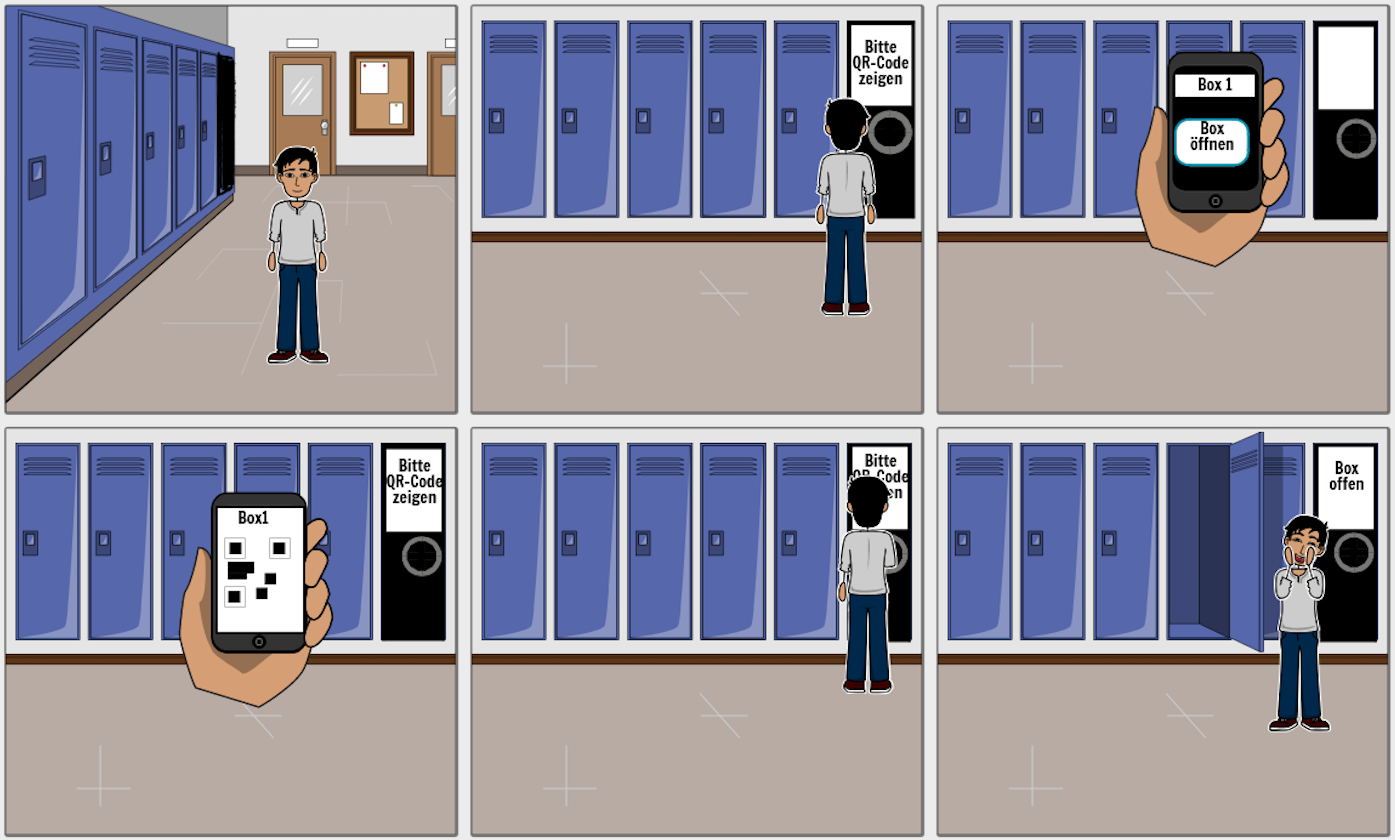
\includegraphics[scale=0.3]{Bilder/Stroyboard.png}
                \captionof{figure}{Stroyboard}
                \footnote{Storyboard erstellt mit StoryboardThat, \url{https://www.storyboardthat.com}}
            \subsubsection{Technische Anforderungen}
                Zur Erfüllung der Nutzeranforderungen lassen sich weitere technische Anforderungen ableiten, die erfüllt werden müssen.
                \begin{itemize}
                    \item Aktualisierungen von Berechtigungen \\ 
                    Im Betrieb des Systems ist es möglich, dass sich die Zugangsberechtigungen ändern. Zum Beispiel können sowohl Nuzter als auch Anbieter eine bestehende Reservierung deaktivieren. In diesem Fall darf die zugehörige Box natürlich nicht geöffnet werden, wenn der zur deaktivierten Reservierung gehörenden QR-Code vorgezeigt wird. Diese Änderung muss also vom Cluster empfangen und die betroffene Reservierung aus der lokalen Datenstruktur entfernt werden. \\
                    Ebenso kann eine deaktivierte Reservierung reaktiviert werden. In diesem Fall muss der zugehörige QR-Code natürlich die entsprechende Box wieder öffnen. Auch dazu muss die Änderung dem Cluster mitgeteilt werden und die betroffene Reservierung der Datenstruktur wieder hinzugefügt werden.
                    
                    \item QR-Code scannen \\
                    Damit ein Nutzer einen QR-Code scannen kann ist es erforderlich, dass die Hardware eine entsprechende Komponente in Form einer Kamera bietet. Auch muss das Kamerabild analysiert und darin enthaltene QR-Codes erkannt sowie in eine Zeichenkette umgewandelt werden. Wurde im Kamerabild ein Qr-Code erkannt und umgewandelt muss außerdem geprüft werden, ob es sich dabei um den Qr-Code einer gültigen Reservierung oder Freigabe für diesen Standort handelt.
                    
                    \item Schloss öffnen \\
                    Wurde im Kamerabild der QR-Code einer gültigen Zugangsberechtigung (Reservierung oder Freigabe) erkannt, so muss die ensprechende Box geöffnet werden. Dazu muss ein Stromkreis entworfen werden, der über die GPIO-Pins des Raspberry Pi ein Relais ansteuert, dass einen 12 Volt Stromimpuls auf das entsprechende Schloss legt und dieses so öffnet.

                    \item Autonomer Start \\
                    Damit das System autonom Hochfahren kann müssen sämtliche Komponenten beim Systemstart automatisch gestertet werden.

                    \item Caching der empfangen Daten \\
                    Damit Nutzer auch im Falle eines Netzwerkausfalls Zugriff auf von ihnen reservierte oder für sie freigegebene Boxen haben werden die Daten zu Boxen, Reservierungen und Freigaben lokal vorgehalten. Zusätlich werden diese Daten auch in Dateien auf der Festplatte persistiert, damit das System in seiner Grundfunktionalität auch verfügbar ist, falls ein Neustart ohne Netzwerkverbindung erforderlich ist.
                \end{itemize}
            
        \subsection{Modelle}
                \subsubsection{Domänenmodell}
                \begin{figure}[h]
                    \centering
                    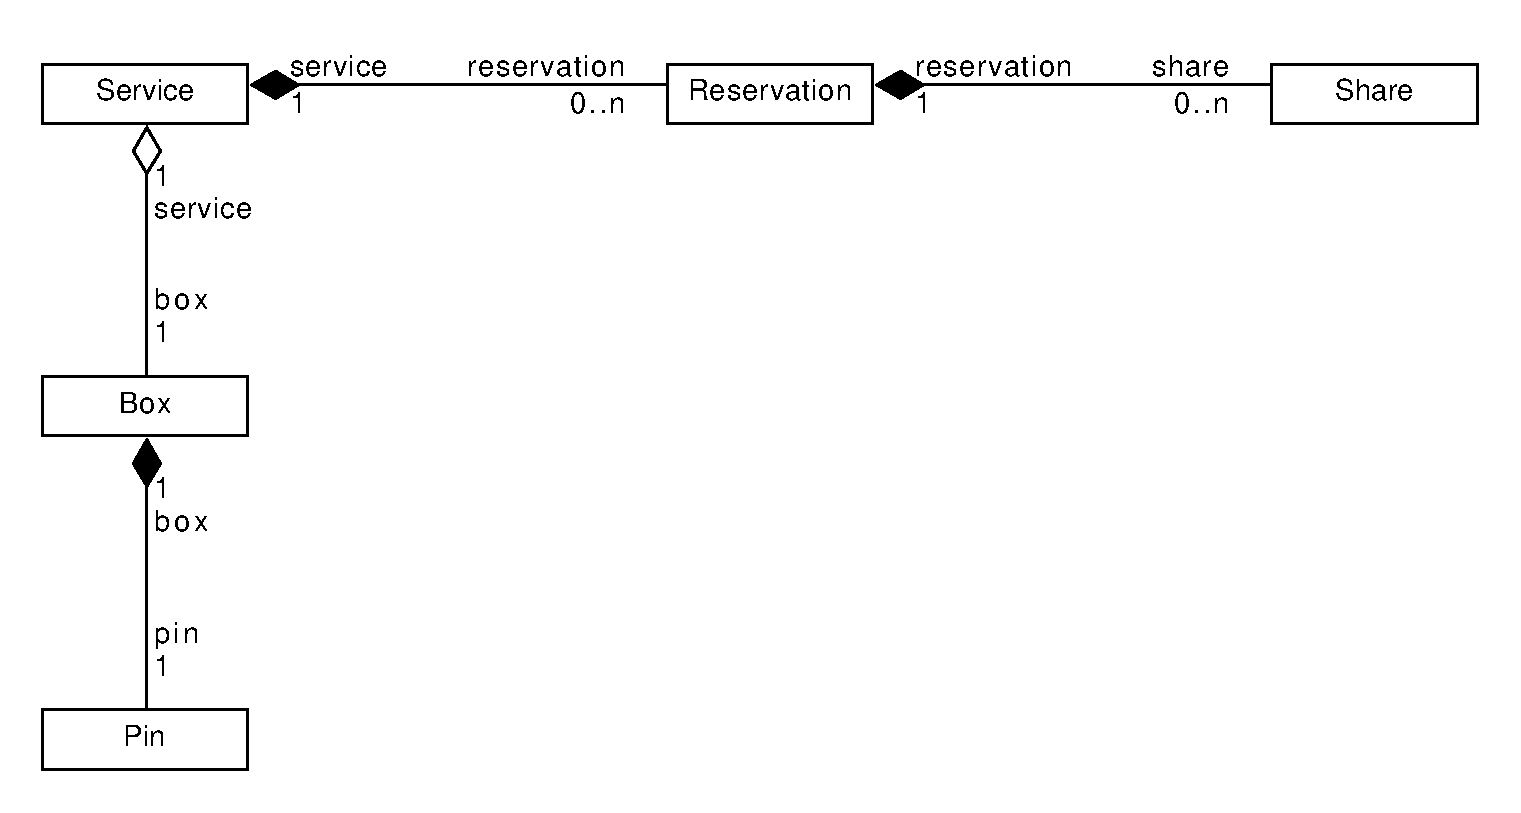
\includegraphics[scale=0.7]{Bilder/Domain_17112019.pdf}
                    \captionof{figure}{Domänenmodell}
                \end{figure}

        \subsection{Architektur}
                \subsubsection{Komponenten}
                    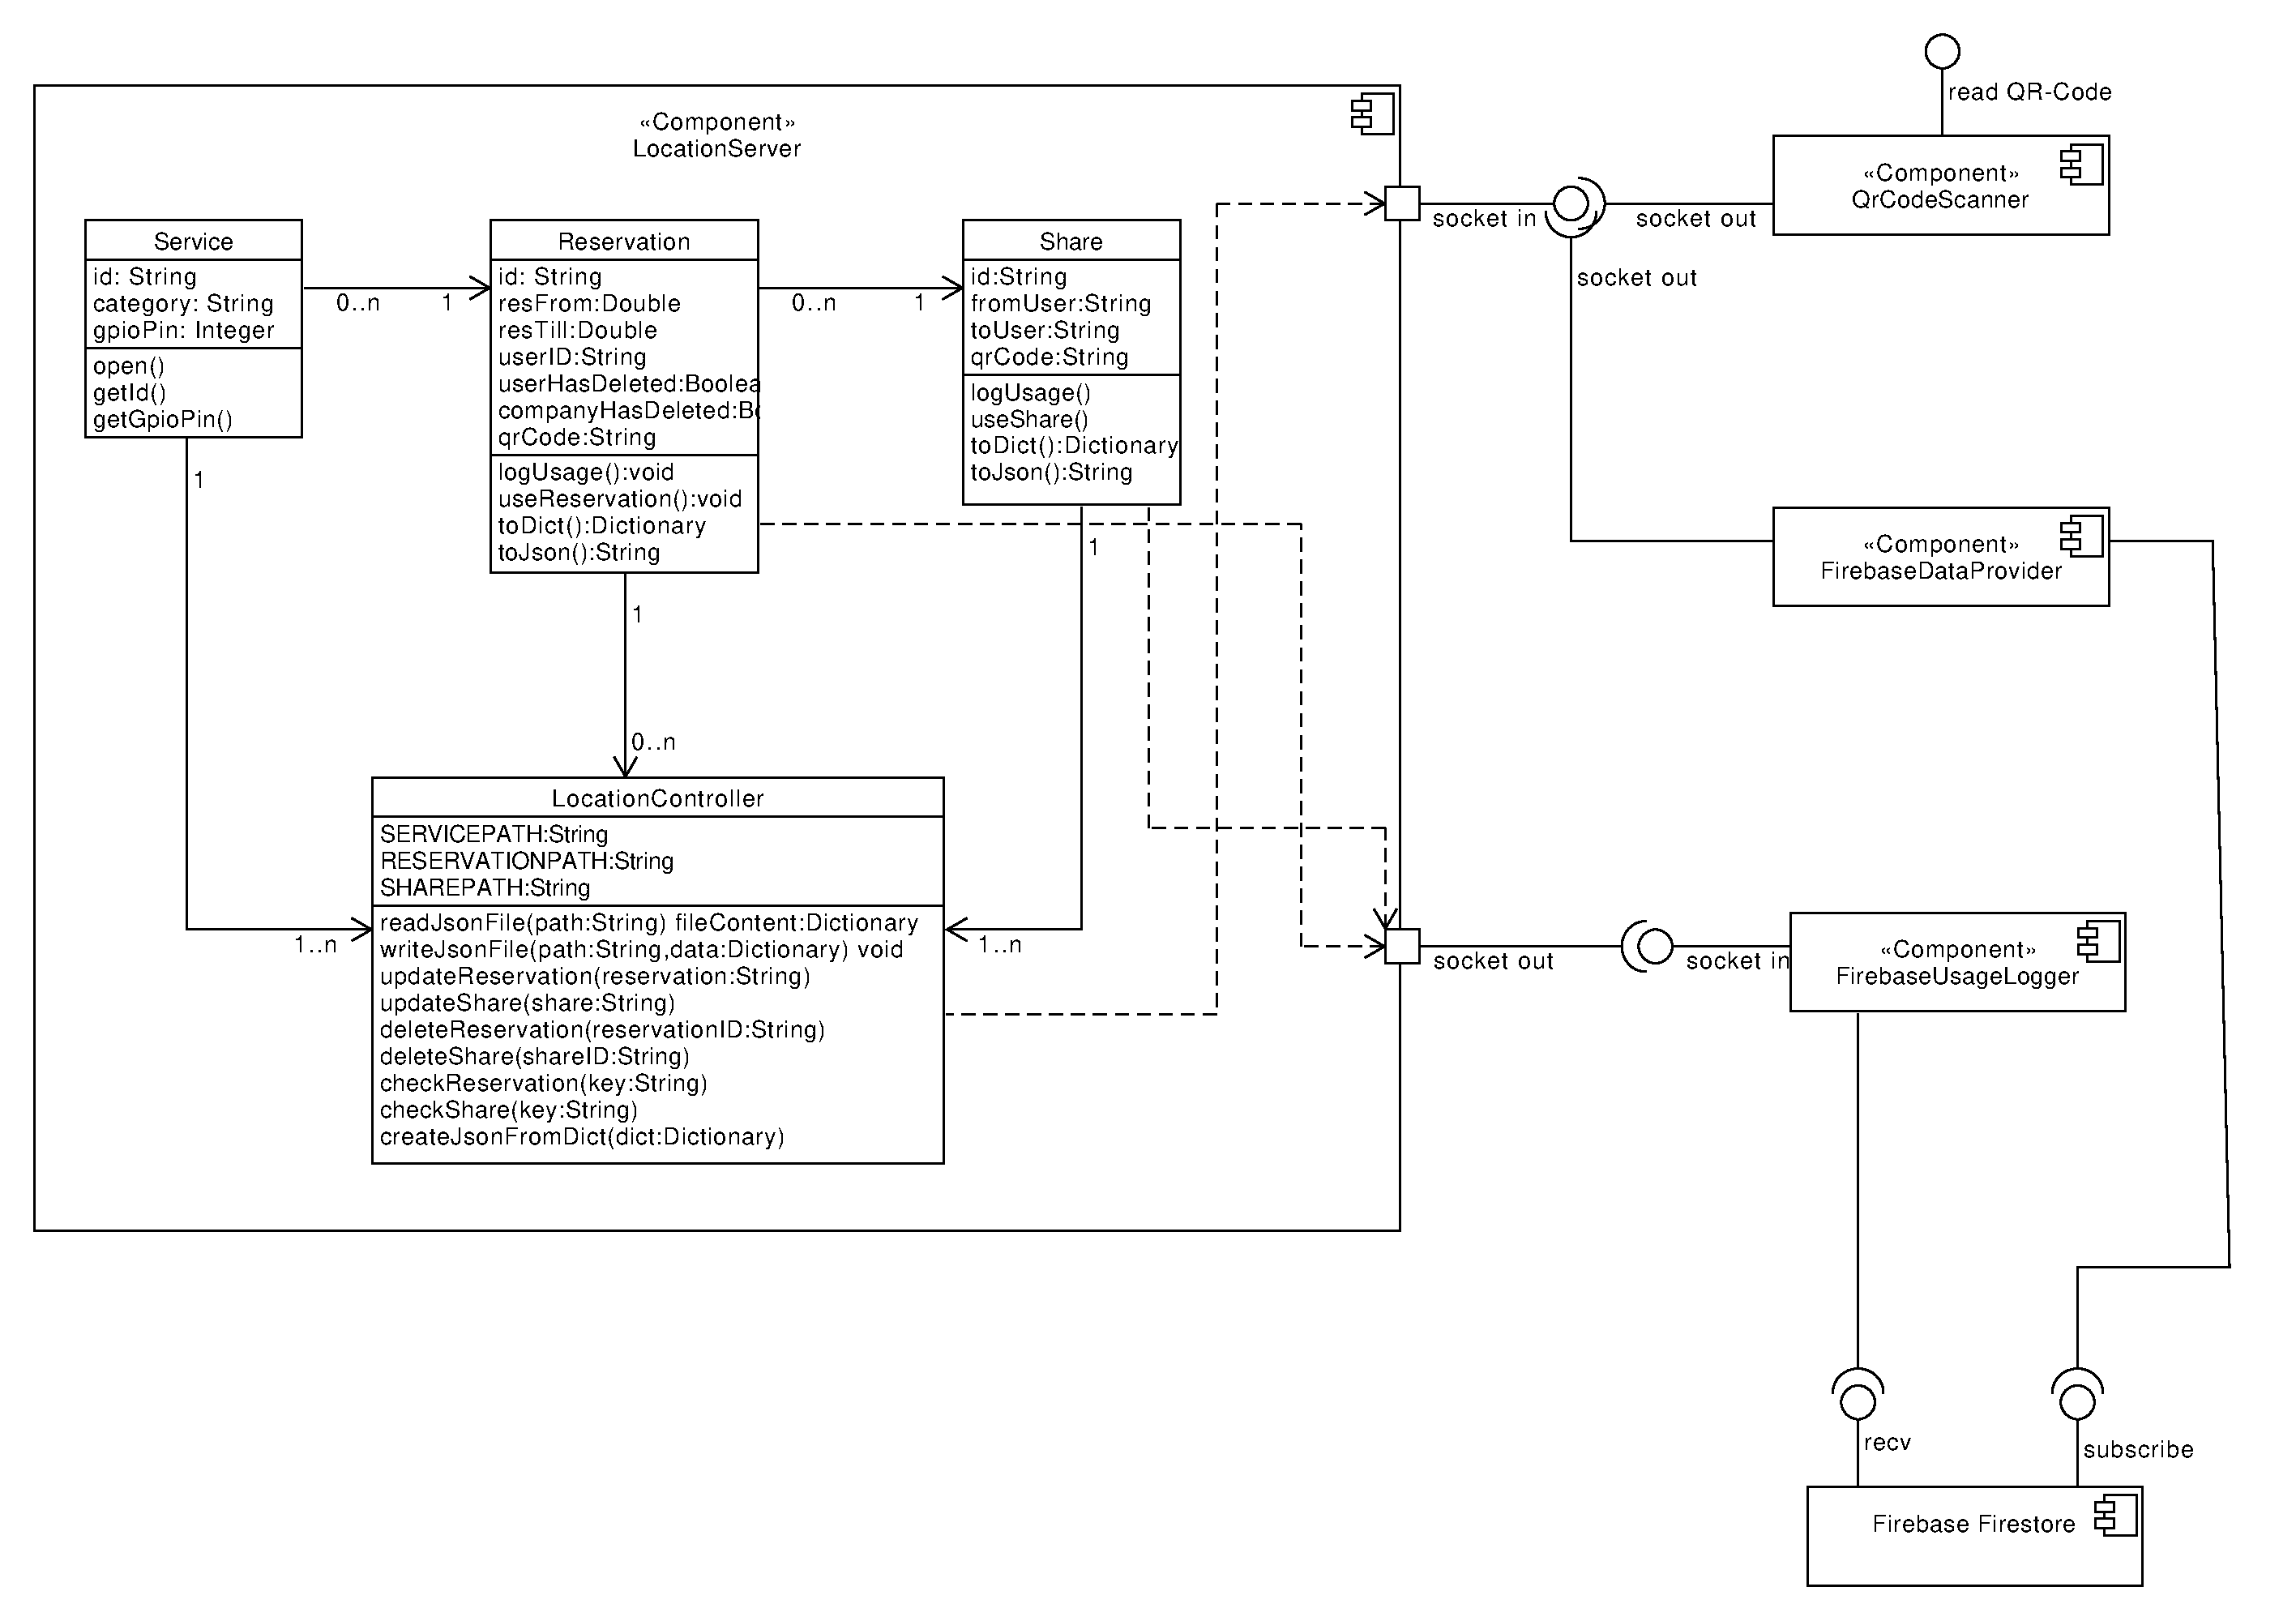
\includegraphics[scale=0.35]{Bilder/Component_16112019.pdf}
                    \captionof{figure}{Komponentendiagramm}
                    
                    Das Softwaresystem besteht aus 4 Komponenten, die die identifizierten Teilprobleme lösen.
                    \begin{itemize}
                        \item LocationServer \\
                        Die Komponente LocationServer ist die zentrale Komponente des System. Sie enthält die Klassen für Services, Reservierungen und Freigaben, sowie mit der Klasse LocationController über eine Klasse zum Speichern, Aktualisieren, Öffnen und Löschen von Services, Reservierungen und Freigaben. \\
                        Sie wird über Unix Sockets von den Komponenten QrCodeScanner und FirebaseDataProvider angesprochen. Ändern sich die Daten für einen Service oder eine Reservierung oder Freigabe, so propagiert die FirebaseDataProvider diese empfangene Änderung an den LocationServer, der die Entsprechenden Methoden der LocationController Klasse aufruft.


                        \item QrCodeScanner \\
                        Bei dieser Komponente handelt es sich um ein Python-Script, dass unter Verwendung der OpenCV- und pyzbar Bibliotheken das Bild der an den Raspberry Pi angeschlossenen Kamera einliest und auswertet.
                        Wird im Kamerabild ein QR-Code gefunden, so wird dieser über einen Unix-Socket an die Komponente LocationServer übergeben um dort ausgewertet zu werden.
                        
                        \item FirebaseDataProvider \\
                        Bei dieser KOmponente handelt es sich um ein NodeJs-Skript, dass für diesen Standort die Daten aus dem Google Cloud Firestore abruft.
                        Dazu ist dem Skript die Adresse des Standortes bekannt. Zunächst werden alle Services abgerufen, die an dieser Adresse vorhanden sind und Listener für diese registriert. Anschließend werden alle Reservierungen für diese Services abgerufen und auch für diese Listener registriert. Zuletzt werden alle Freigaben für diese Reservierungen abgerufen und auch für diese Listener registriert. Werden nun für diesen Standort neue Services angelegt oder treten in Reservierungen oder Freigaben von Services an diesem Standort Änderungen auf, so teilt Google Cloud Firestore diese Änderungen dem FirebaseDataProvider mit, welcher sie Änderungen wiederrum an den LocationServer weitergibt.
                        \item FirebaseUsageLogger \\
                        Die Aufgabe dieser Komponenten besteht darin, im Faller einer Öffnung eines Services über eine Reservierung oder Freigabe diese Öffnung an das Google Cloud Firestore Backend zu übermitteln.
                        Dazu werden ihr die Daten von der betreffenden Reservierung oder Freigabe über den Unix-Socket mitgeteilt, mit einem Zeitstempel versehen und an die Google Cloud Firestore Datenbank zurückgeschrieben.
                        Die mitgeteilten Daten bestehen aus der ID der REservierung oder Freigabe, der ID des Nutzers und der den Service göffnet hat.
                    \end{itemize}
            \subsection{Abläufe}
                    \subsubsection{Reservieren einer Box}
                        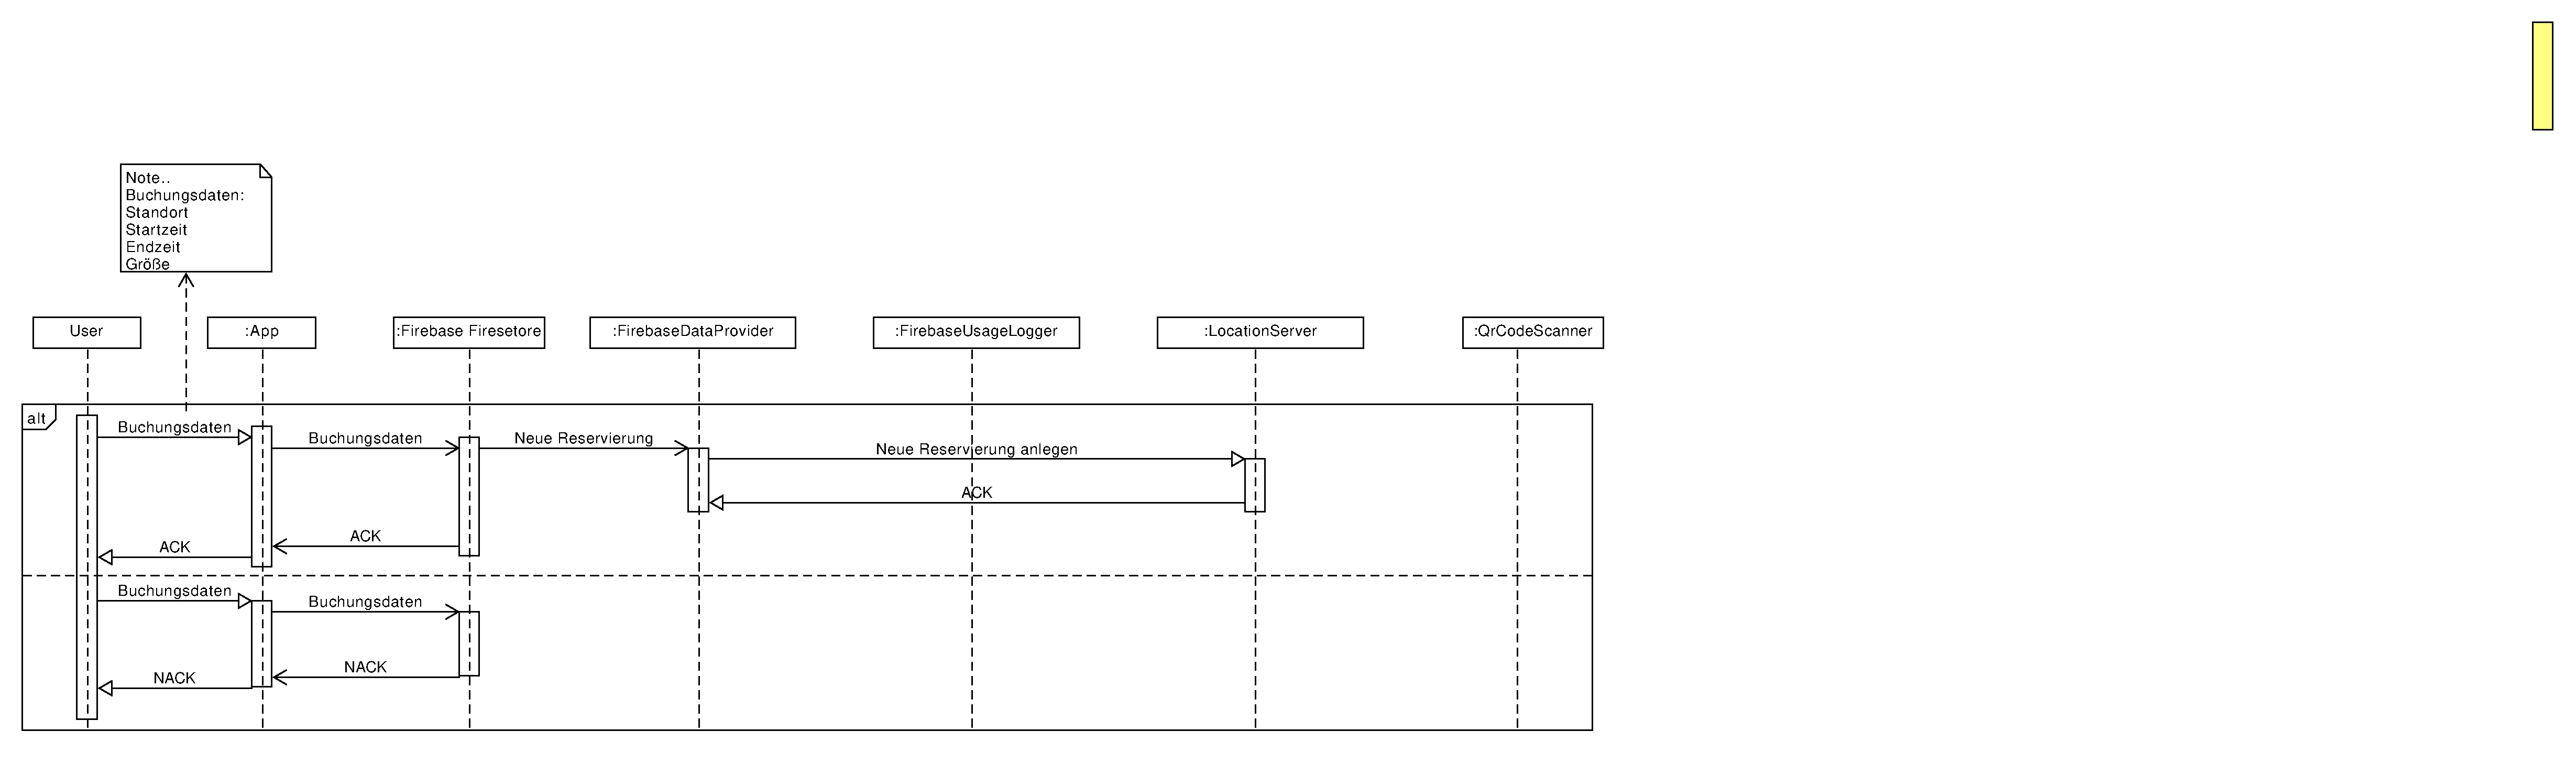
\includegraphics[scale=0.32]{Bilder/Rent_Sequence_14112019.pdf}
                        \captionof{figure}{Reservieren}
                    \subsection{Öffnen einer Box}
                        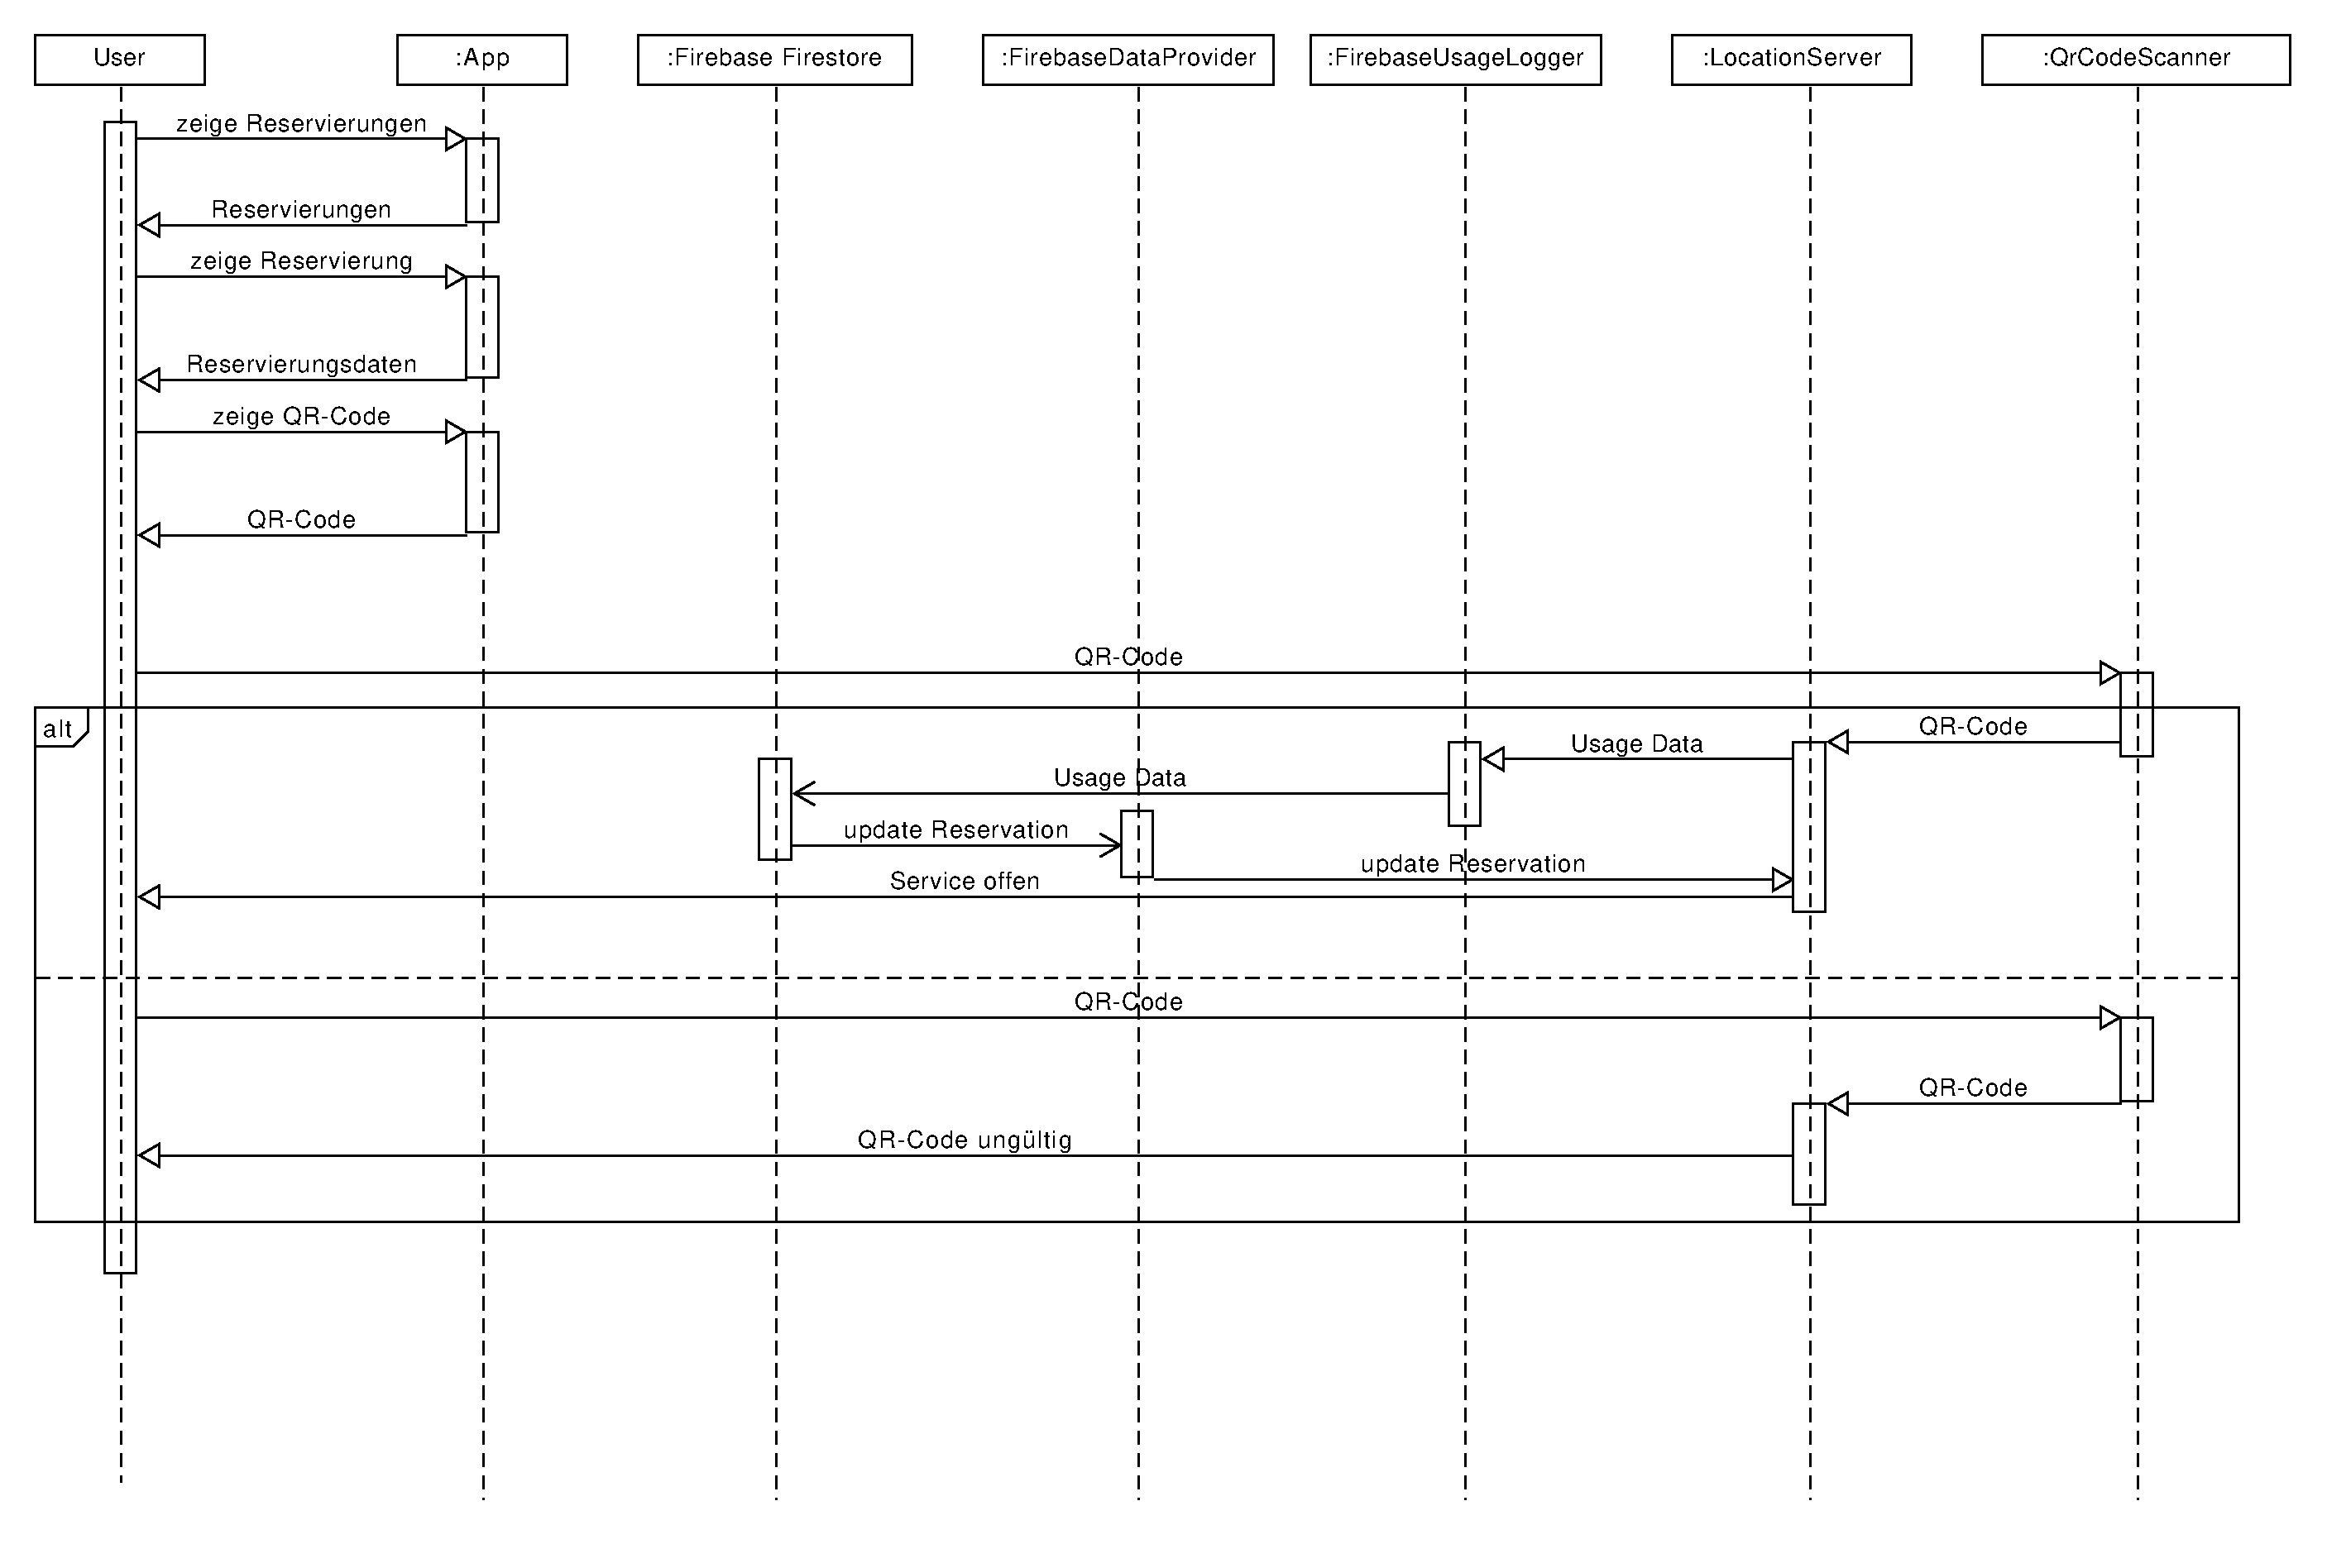
\includegraphics[scale=0.32]{Bilder/Open_Reservation_Sequence_15112019.pdf}
                        \captionof{figure}{Öffnen der Box mit einer Reservierung}


    \section{Fazit}

    \section{Ausblick}
    
    \bibliography{aux/literatur.bib}
    \bibliographystyle{alpha}
\end{document}